\chapter{Models}
\section{Grammatical Parse} \label{section:gramaticalParse}
After consultation with British Fencing, I was directed to a useful resource
which describes how fencing competitions operate \citep{bf-comp-guide}. Not
all of this document is relevant but the sections that are are reproduced
below, with \textbf{nouns} in bold and \underline{verbs} underlined. Only the
nouns and verbs deemed to be directly relevant to the process of competing in a
competition have been included.
\begin{displayquote}
Check In: All \textbf{competitions} start by \textbf{fencers}
visiting the \textbf{check in desk} \underline{to confirm} that they
are present. Don’t miss this bit out - your \textbf{entry}
will \underline{be scratched}.
When \underline{checking in}, \textbf{fencers} are required to show
their \textbf{British Fencing card}. See the box (right) for
details. This carries \textbf{insurance}. Without it, you
may not fence. Fencing usually starts about 30 - 60 minutes
after \underline{check in} closes.
Pools: After \textbf{check in}, \textbf{competitors} are divided
into “\textbf{pools}” - groups of 5 - 7 \textbf{fencers} who all
\underline{fence} each other up to 5 \textbf{hits}. (4 \textbf{hits} for some
under 9 \textbf{competitions}). Time is limited to 2 or 3
minutes. Sometimes there may be two rounds of
\textbf{pools}, particularly in \textbf{age group competitions}.
Direct Elimination: The \textbf{results} of the \textbf{pools}
are used to \underline{seed} the \textbf{knockout phase} of the
\textbf{competition}. In some \textbf{competitions}, up to 30\%
of the \textbf{fencers} who did worst are \underline{eliminated}, but
in most cases all \textbf{fencers} \underline{go through} to the \textbf{direct
elimination (DE)} stage.
The \textbf{DE} rewards \textbf{fencers} who do well in the
\textbf{pool} stages, and keeps the strong \textbf{fencers} apart
until near the end of the \textbf{competition}. In a
\textbf{competition} with 64 \textbf{entrants}, the first round of
DEs would see 1st place fence 64th, 2nd place
fence 63rd and so on. If the number of
\textbf{entrants} is not a power of 2, (ie 8, 16, 32, 64
etc) then those \textbf{fencers} who did best in the \textbf{pools}
will \underline{get a “\textbf{bye}”} through the first \textbf{DE} round. After
several \textbf{DE} rounds, there will only be two \textbf{fencers}
left - the \textbf{finalists}.
\textbf{Direct elimination} fights are up to 15 \textbf{hits} (adults)
10 \textbf{hits} (under 13s) or 8 \textbf{hits} (under 9s). \textbf{DE fights}
are normally 3 x 3 minutes (sometimes less for \textbf{younger
fencers}) with a 60 second break between \textbf{periods}.
\end{displayquote}
\section{Project Glossary} \label{section:projectGlossary}
From the grammatical parse in section \vref{section:gramaticalParse} a project
glossary can be compiled. As a part of this, I removed all duplicate words, plurals and synonyms, chosing the most
appropriate word from any sets of synonyms as the noun or verb to represent
that entity/action. Note that synonyms in this sense are not necessarily true
synonyms but are equivalent terms in the context of fencing and fencing
competitions. Objects that have been identified as being a synonym of another
object, but not a complete synonym have had \textit{(sub-type)} appended to them
in the synonym list. The description of the words comes either from the text
above, from basic internet searching, or from my own knowledge of the sport.
\begin{center}
\begin{longtable}[l]{| p{.20\textwidth} | p{.80\textwidth} |} 
 \caption{\label{tab:ProjectGlossary}Project Glossary}
 \hline
 \textbf{Nouns} & \\ 
 Competition & An over-arching event at which one or more events
 take place \\
 & \textit{synonyms: age group competition (sub-type)} \\ 
 Fencer & An individual (human being) who competes in a fencing
 competition \\
 & \textit{synonyms: competitor, entrant, finalists (sub-type),
 younger fencers (sub-type)} \\
 Check-in desk & The location that fencers present themselves to
 in order to confirm that they will take part in a competition \\
 Entry & The link between a fencer and a competition \\
 British Fencing Card & A form of identity card indicating that a
 fencer has membership of British Fencing, and by extension is insured to
 compete \\
 & \textit{synonyms: insurance} \\
 Hit & The act of one fencer striking another and scoring a point \\
 Result & A listing of fencers in order of their measured performance in a 
 particular round \\
 Direct Elimination & The phase of a competition where defeating
 another fencer results in their elimination from the competition and your
 promotion to the next round. \\
 & \textit{synonyms: DE, knockout phase} \\
 Bye & The act of progressing through a round of the Direct
 Elimination stage of the competition without having to face another fencer.
 This is used in the event that the number of fencers is not a power of 2. \\
 Bout & An individual fencing match between two fencers \\
 & \textit{synonyms: fight} \\
 Period & A time-based subdivision of a bout \\
 Poule & A small grouping of fencers who all fence against one
 another in a series of bouts. \\
 & \textit{synonyms: pool} \\ 
 Event & A tournament in which fencers of the same gender, age
 group and weapon fence \\
 \textbf{Verbs} & \\
 Check In & The act of a fencer confirming that they have arrived at the venue
 of the competition and they intend to compete in it. \\
 & \textit{synonyms: to confirm (attendance at the competition)} \\
 Be Scratched & To be removed from the competition without competing \\
 Fence & The act of one fencer engaging in a fencing bout with another fencer \\
 & \textit{synonyms: fight} \\
 Seed & To use the results of one or more round(s) of competition to determine
 the structure of the next round. \\
 Eliminated & To be removed from the competition as a result of loosing a bout
 in a Direct Elimination round, or (in some cases) not being ranked high enough
 after a round of Poules \\
 Go Through & To progress from one round to the next, either by being ranked
 high enough after a poules round, or by winning a Direct Elimination bout \\
 Get a Bye & Be in receipt of free passage from one round of Direct
 Elimination to the next, without having to face another fencer. This is used in
 the case that the number of competitors in a round of Direct Elimination is not
 a power of 2 \\
 \hline
\end{longtable}
\end{center}
\section{Business Processes} \label{section:businessProcesses}
I have decided that for the purposes of this project, modelling the business
processes associated with the process of a fencer taking part in a competition
is not appropriate. The reason for this is that the software system will not
seek to implement these processes, but rather be an archive or the results of
these processes. Other software (such as Engarde and Fencing Time, mentioned in
section \vref{chapter:research}) already implement these processes. The
business processes that I will model will be the process by which data gets
added to the system and viewed by users of the system.
\section{Class Diagram}
As mentioned above, the project glossary includes terms relating to the actual
competition process. Some of these terms are relevant to a results hosting
service and some are not. Terms like \textit{Check-in desk} and
\textit{British Fencing Card } are only relavent during the actual competition
itself, therefore I have excluded them from the class diagram below.
\begin{figure}[!ht]
    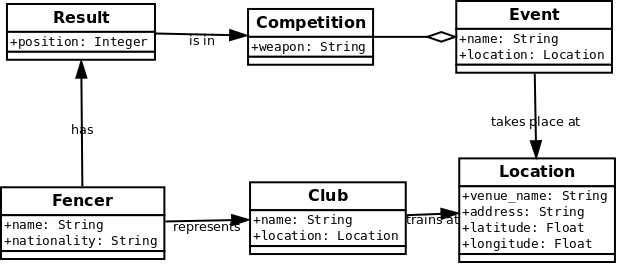
\includegraphics[width=\textwidth]{class_diagram}
    \caption{Class Diagram}
  \end{figure}